\chapter{XMPP}\label{chap:6}
\section{Servicios de Mensajería}
\subsection{Introducción}

En esta práctica se utilizará el protocolo XMPP.
Se utiliza un docker para almacenar el servidor XMPP.
Los alumnos crean clientes para interactuar en el servidor mediante mensajes XMPP.
Finalmente, se estudia algún aspecto del protocolo y se desarrolla un bot.

\begin{notebox}
Todos los ficheros y configuraciones relacionadas a esta sesión se encuentran en el directorio
\lstinline{is-pl3-g1/6_xmpp}.
\end{notebox}

\subsection{Servidores XMPP}

La primera tarea a realizar es instalar el servidor XMPP es un contenedor Docker.
Posteriormente, hemos configurado el fichero \lstinline{prosody.cfg.lua} 
(localizado en \lstinline{etc/prosody/prosody.cfg.lua}).
Escribimos el fichero \lstinline{Dockerfile} que lanza el contenedor de Prosody,
pasándole las carpetas de configuración \lstinline{data} y \lstinline{etc/prosody}.
A continuación, hemos creado los certificados necesarios para el servidor, y los extraemos
del contenedor Docker a nuestra carpeta de configuración \lstinline{data} (\lstinline{ingserv01.*}).

Finalmente, hemos dado de alta a dos cuentas de usuario en el servidor Prosody
para que puedan acceder a la aplicación XMPP.

Los dos usuarios son:
\begin{itemize}[itemsep=0.10px]
    \item manolo@ingserv01 (conManolo)
    \item ramon@ingserv01 (conRamon)
\end{itemize}

\subsection{Clientes XMPP}

En la distribución de Linux utilizada para instalar el cliente, Debian 12 Bookworm,
se han instalado los paquetes del repositorio oficial \italic{stable}
\lstinline{pidgin 2.14.12-1} y \lstinline{pidgin-data 2.14.12-1}.

\begin{minipage}{\linewidth}
	\centering
	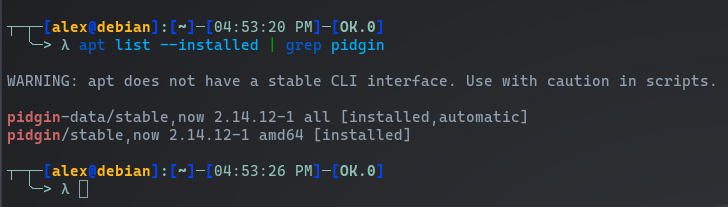
\includegraphics[width=0.8\textwidth]{6/Imagen610.png}
	\captionof{figure}{Paquetes a instalar en Debian 12 Bookworm}\label{fig:6/1}
\end{minipage}

Mediante las herramientas de desarrollador, se aprecia que se descargan fragmentos del vídeo

Hacemos login como ambos usuarios y los añadimos como amigos.
De ahora en adelante, será posible que estos dos usuarios chateen entre ellos.

\begin{minipage}{\linewidth}
	\centering
	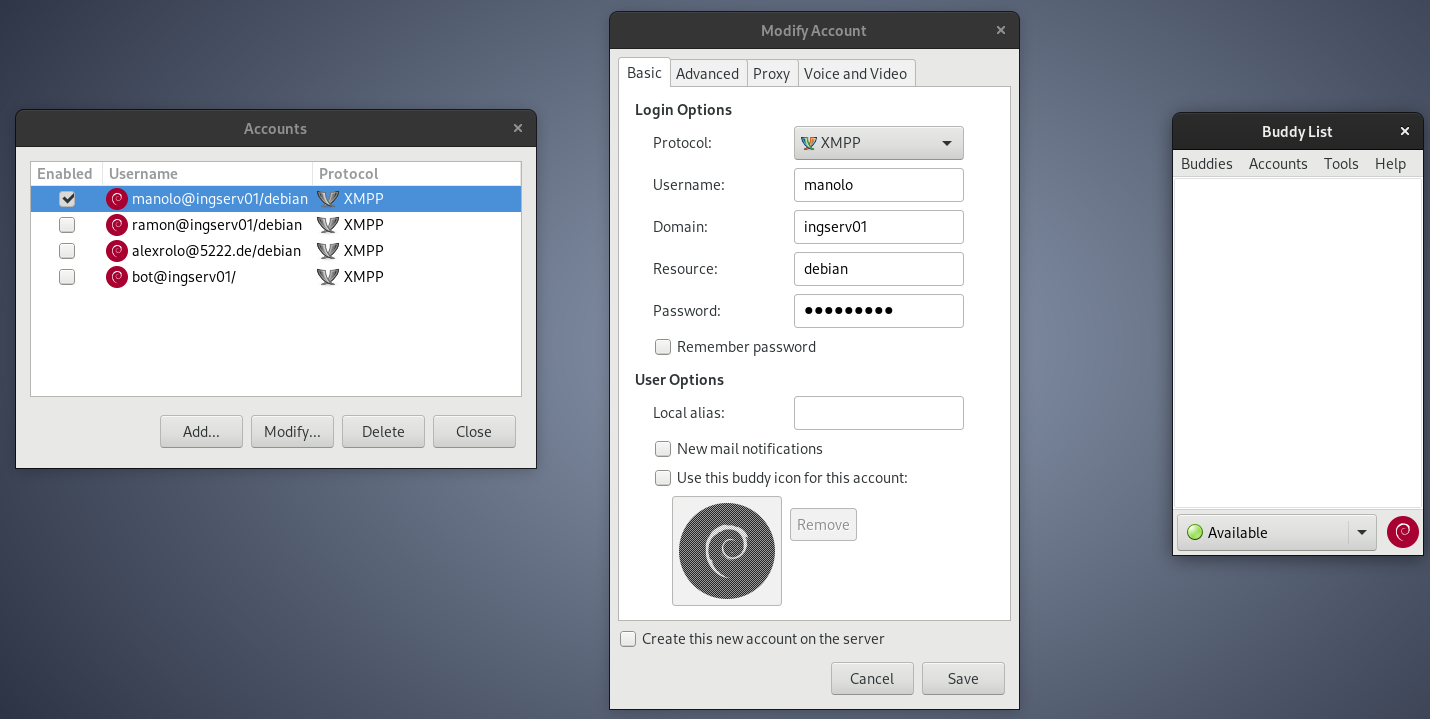
\includegraphics[width=0.8\textwidth]{6/Imagen611.png}
	\captionof{figure}{Login con uno de los usuarios}\label{fig:6/2}
\end{minipage}

Estos dos usuarios se comunican utilizando el programa.

\begin{minipage}{\linewidth}
	\centering
	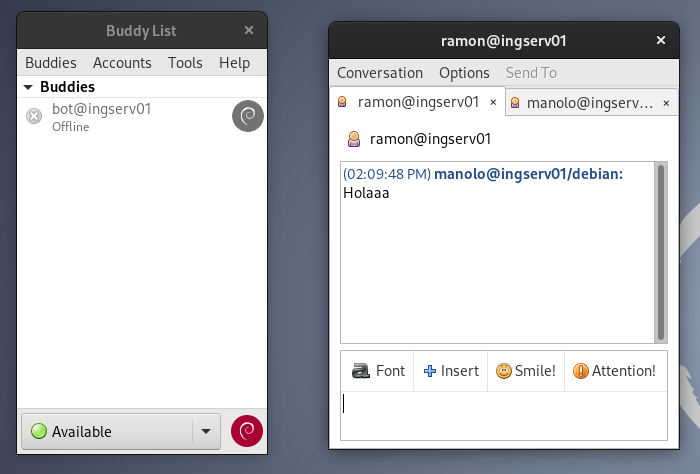
\includegraphics[width=0.8\textwidth]{6/Imagen613.png}
	\captionof{figure}{Chat entre dos usuarios}\label{fig:6/3}
\end{minipage}

\subsection{Protocolo XMPP}

Procedemos a analizar las \italic{stanzas} que recibe la app Pidgin.
Podemos ver las estrofas del \lstinline{ping} que envía Pidgin periódicamente.
También se ven los cambios de estado con la \italic{stanza} presence.
Finalmente, observamos \italic{stanzas} recibidas al enviar un mensaje.

\begin{minipage}{\linewidth}
	\centering
	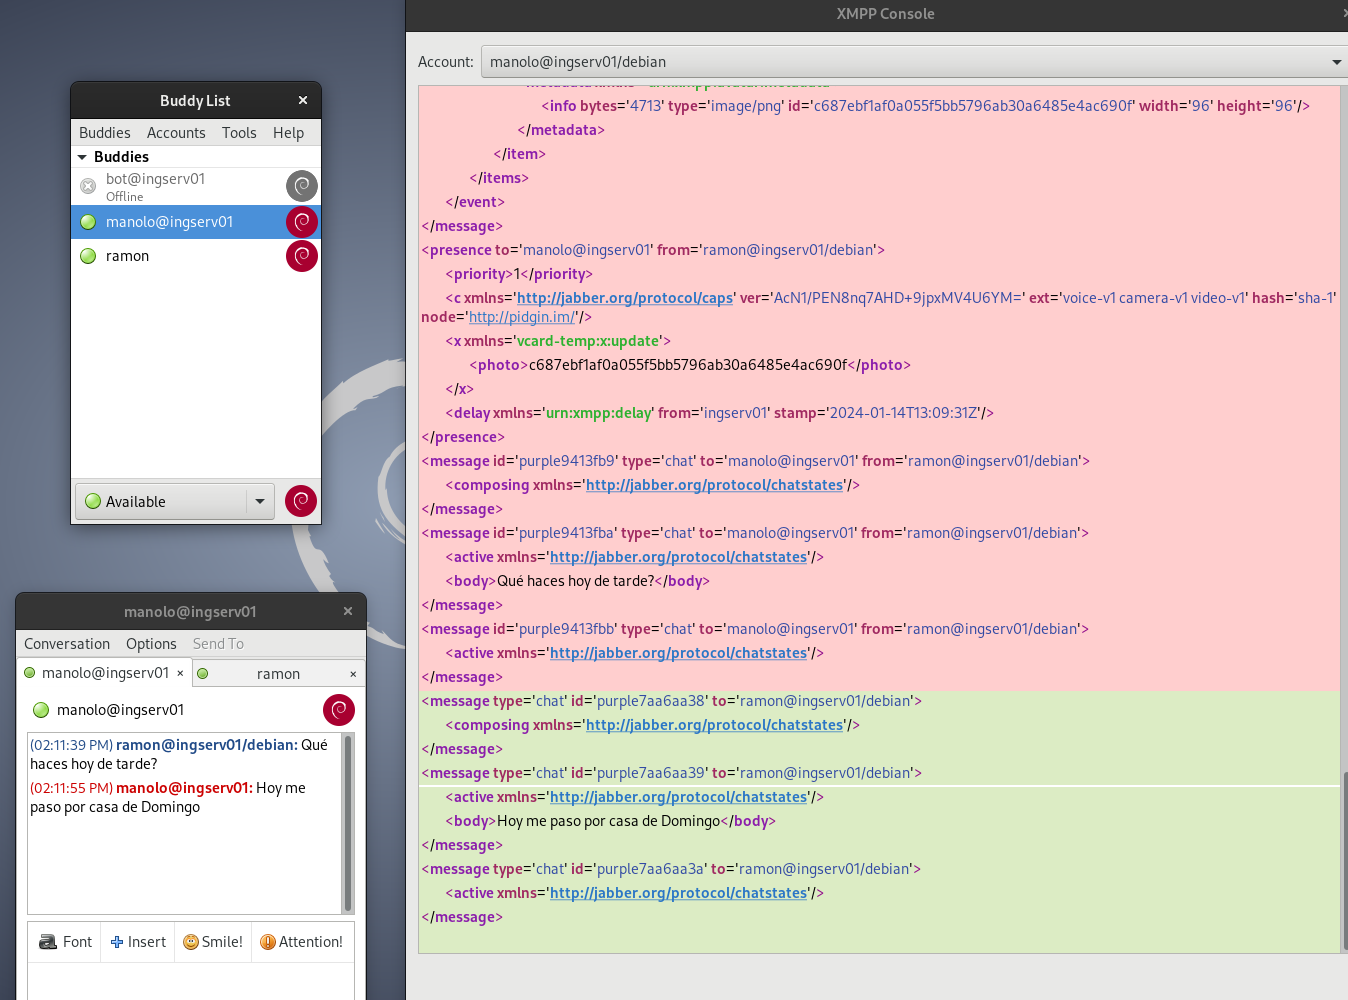
\includegraphics[width=0.8\textwidth]{6/Imagen612.png}
	\captionof{figure}{Mensajes entre dos usuarios}\label{fig:6/4}
\end{minipage}

Igual sucede cuando dos usuarios se subscriben a las notificaciones.

\begin{minipage}{\linewidth}
	\centering
	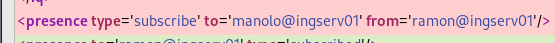
\includegraphics[width=0.8\textwidth]{6/Imagen614.png}
	\captionof{figure}{Subscripción de un usuario a otro}\label{fig:6/5}
\end{minipage}

\subsection{Bot XMPP}

En esta ultima sección desarrollamos un bot XMPP.
El bot funcionará como un usuario más en el roster.
Usuarios podrán añadir al bot a su lista de amigos y le podrán enviar mensajes.
Si al bot se le presenta una operación matemática, responderá con el resultado,
mientras que si no es una operación matemática, el bot responderá con el mismo mensaje.

A la hora de desarrollar el bot, nos encontramos con varios problemas.
La libería a utilizar, \lstinline{sleekxmpp} no estaba disponible en el repositorio
oficial de Debian y el script de instalación del paquete de \lstinline{pip} no funciona correctamente.

Como solución a este problema, decidimos omitir la tarea de desarrollar el bot en local
y proceder directamente a desarrollar el bot en un contenedor Docker.

Al utilizar un contenedor Docker, podemos bajarnos una imagen de una versión de Python que sí soporte
el paquete de \lstinline{pip sleekxmpp}.

El \lstinline{Dockerfile} utiliza una imagen de \lstinline{Python 3.8}
y los paquetes \lstinline{wheel} y \lstinline{sleekxmpp}.

Una vez hecho esto, hemos comenzado el desarrollo del bot.
Definimos la clase \lstinline{Bot} y sus métodos de \lstinline{callback}.
Añadimos un método \lstinline{main} que crea una nueva instancia del bot
y solicita los parámetros necesarios si no se han pasado previamente
por línea de comandos.

Hemos tenido que añadir dos líneas de código específicas sobre \lstinline{SSL}
para que el bot ignore el certificado del servidor.
Si no se añaden estas líneas, nos es imposible ejecutar el bot con exito.

Finalmente, escribimos un fichero \lstinline{lanza-bot.sh} con el código necesario
para lanzar el contenedor del bot e iniciar el programa con los parámetros adecuados.

Aquí se muestra un ejemplo de interacción con el bot:

\begin{minipage}{\linewidth}
	\centering
	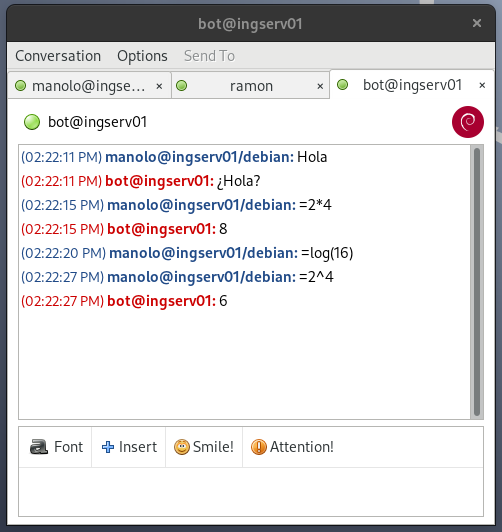
\includegraphics[width=0.8\textwidth]{6/Imagen615.png}
	\captionof{figure}{Comunicación con el bot}\label{fig:6/6}
\end{minipage}

No obstante, al enviar el mensaje \verb#=log(16)#
el bot no sabe qué hacer, por lo que la función \verb#eval#
que utilizamos para resolver las operaciones no tiene todas
las funciones matemáticas definidas.

\begin{minipage}{\linewidth}
	\centering
	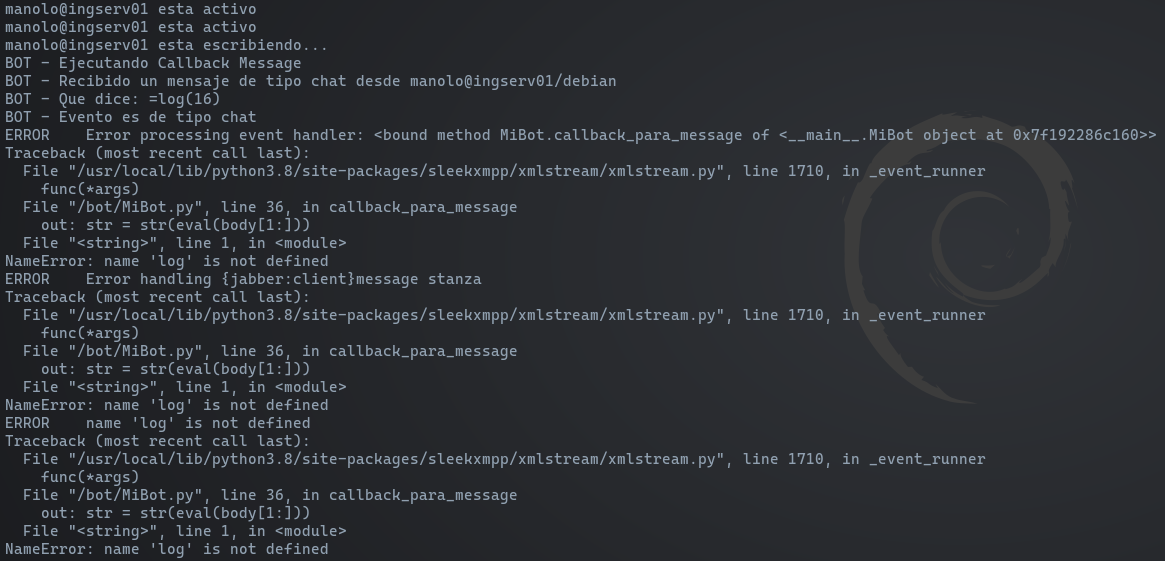
\includegraphics[width=0.8\textwidth]{6/Imagen616.png}
	\captionof{figure}{Excepción en el bot al usar $log$}\label{fig:6/7}
\end{minipage}
